\documentclass[12pt]{article}
%
%
% Retirez le caractere "%" au debut de la ligne ci--dessous si votre
% editeur de texte utilise des caracteres accentues
%\usepackage[latin1]{inputenc}
\usepackage[utf8]{inputenc}

%
% Retirez le caractere "%" au debut des lignes ci--dessous si vous
% utiisez les symboles et macros de l'AMS
\usepackage{amsmath}
\usepackage{amsfonts}
%
%
\setlength{\textwidth}{16cm}
\setlength{\textheight}{21cm}
\setlength{\hoffset}{-1.4cm}

% for figures and tables
\usepackage{float}
\usepackage{graphicx}
\usepackage{wrapfig}
\usepackage{xcolor}
\usepackage{hyperref}
\hypersetup{
	colorlinks,
	linkcolor=black,
	urlcolor=violet
}
\usepackage{scrextend}
%
%
\begin{document}

%--------------------------------------------------------------------------

\begin{center}
{\Large
	{\sc Parallélisation de l'algorithme des $k$-médoïdes. Application au clustering de courbes.} %heuristique ?!
}
\bigskip

Benjamin Auder $^{1}$ \& Jairo Cugliari $^{2}$
\bigskip

{\it
$^{1}$ Laboratoire LMO. Université Paris-Sud. Bât 425. 91405 Orsay Cedex, France.\\benjamin.auder@math.u-psud.fr

$^{2}$ Laboratoire ERIC. Université Lumière Lyon 2. Bât K. 69676 Bron Cedex, France.\\jairo.cugliari@univ-lyon2.fr
}
\end{center}
\bigskip

%--------------------------------------------------------------------------

{\bf R\'esum\'e.} 
Nous présentons une méthode de clustering adaptée à de grandes bases de données de courbes densément discrétisées, donc elle-mêmes en grande dimension. 
La classification obtenue peut être utilisée afin de choisir de meilleurs modèles de prédiction de courbes, plus spécifiques, dans chacun des groupes. 
La méthode consiste en deux principales étapes : 
réduire la dimension des courbes via une base d'ondelettes, puis effectuer le clustering en parallèle. 
Les ondelettes sont bien adaptées pour identifier des caractéristiques localisées en temps et échelle. 
De plus, l'aspect multi-résolution de la transformée en ondelettes permet de regrouper les coefficients 
selon leur contribution à l'énergie totale, fournissant ainsi des représentants compacts pour chaque courbe. 
L'algorithme des $k$-médoïdes est appliqué à plusieurs sous-échantillons de l'ensemble des représentations réduites, 
puis les centres finaux sont obtenus en recherchant la médiane (ou éventuellement la moyenne) des médoïdes des échantillons. 
Des applications sont présentées sur deux jeux de données, dont les consommations électriques irlandaises journalières.
\smallskip

{\bf Mots-cl\'es.} réduction de dimension, ondelettes, $k$-médoïdes, parallèle
\bigskip\bigskip

{\bf Abstract.}
We present a clustering method adapted to large databases of densely sampled curves, hence themselves in high dimension. 
The resulting classification can help to better tune models to predict new curves, each in every group. 
The method consists of two main steps: 
use a wavelet basis to reduce curves dimensionality, and then run a parallel clustering algorithm. 
Wavelets are well suited to identify characteristics localized both in time and space. 
Moreover, the multiresolution nature of the wavelets transform allows to group coefficients according to their 
contribution to the total energy, thus providing compact representations for every curve. 
The $k$-medoids algorithm is applied to several subsamples of all the reduced representations, and then the final 
centers are obtained by computing the median (or mean) of the samples medoids. 
Applications are shown on two databases, including Irish daily electrical consumptions.
\smallskip

{\bf Keywords.} dimensionality reduction, wavelets, $k$-medoids, parallel

%~ Nous présentons une méthode de clustering adaptée à de grandes bases de données de courbes densément discrétisées, donc elle-mêmes en grande dimension. La classification obtenue peut être utilisée afin de choisir de meilleurs modèles de prédiction de courbes, plus spécifiques, dans chacun des groupes. La méthode consiste en deux principales étapes : réduire la dimension des courbes via une base d'ondelettes, puis effectuer le clustering en parallèle. Les ondelettes sont bien adaptées pour identifier des caractéristiques localisées en temps et échelle. De plus, l'aspect multi-résolution de la transformée en ondelettes permet de regrouper les coefficients selon leur contribution à l'énergie totale, fournissant ainsi des représentants compacts pour chaque courbe. L'algorithme des k-médoïdes est appliqué à plusieurs sous-échantillons de l'ensemble des représentations réduites, puis les centres finaux sont obtenus en recherchant la médiane (ou éventuellement la moyenne) des médoïdes des échantillons. Des applications sont présentées sur deux jeux de données, dont les consommations électriques irlandaises journalières.

%--------------------------------------------------------------------------

\section{Introduction}

% * clustering
% * parallelisation of clustering
% * fda + wavelets
% * données individuelles de conso

Récemment, le contexte du \textit{Big Data} a rendu nécessaire le développement d'algorithmes spécifiques à de (très) 
grands volumes de données, éventuellement aussi en grande dimension comme c'est le cas dans notre étude. 
Ainsi ont vu le jour des algorithmes opérant sur de grands graphes (Kang et al.~2009) ou sur des flux de données haut débit (De Francisci Morales et Bifet~2013), entre entres. 
Le livre de Bekkerman et al.~(2011) présente des algorithmes de Machine Learning s'exécutant en parallèle sur diverses architectures, et 
ce type de programmation est en plein essor.\\

\noindent La classification non supervisée (\textit{clustering}) est une des branches de l'apprentissage non supervisé. 
L'objectif est de regrouper les données en \textit{clusters} homogènes, suffisamment distincts deux à deux. 
Depuis la proposition originale de Tyron~(1939) un grand nombre d'articles ont été publié à ce sujet (voir Berkhin~2006 pour une revue). 
Cependant, il n'y a pas de consensus sur la définition d'un cluster : celle-ci varie en fonction des données, du contexte et de l'algorithme utilisé. 
Malgré ce fait, la classification non supervisée reste une technique très populaire qui permet 
de réduire la taille des données en les résumant à quelques représentants ; c'est particulièrement intéressant lorsqu'on travaille sur de grosses bases de données.\\

\noindent Dans ce travail nous avons choisi d'adapter un algorithme de clustering classique pour une exécution parallèle, opérant sur des données de dimension réduite. 
La première partie présente la technique retenue afin d'abaisser la dimension via une base d'ondelettes. 
L'algorithme classant les données en parallèle est expliqué dans la seconde partie, puis nous montrons quelques résultats de tests.

\section{Réduction de dimension}

Dans cette section nous expliquons comment sont traitées les variables fonctionnelles (voir Antoniadis et al.~(2013) pour plus de détails).\\

\noindent Chaque fonction $z$ est d'abord discrétisée sur une fine grille (toutes les 30 minutes pour les consommations électriques), et 
la discrétisation est encore notée $z = \{ z(t_i), i = 1, \ldots, N \}$. 
$z$ est alors approchée (jusqu'à l'échelle $J$) par un développement tronqué sur une base d'ondelettes avec un coefficient d'échelle $c_{0,0}$ 
et les coefficients d'ondelettes $\{d_{j, k}\}_{j, k}$ :
%
\begin{equation} \label{approx}
    z_J(t) = c_{0,0} \phi_{0, 0} (t) + \sum_{j=0}^{J-1} \sum_{k=0}^{2^j - 1} d_{j,k} \psi_{j, k} (t).
\end{equation}
Alors, l'énergie $\mathcal{E}_Z =  \| z \|^2_{ L_2 }$ de chaque fonction $z$ est égale à la somme des énergies 
de ses coefficients en ondelettes distribuées à travers les échelles :
%
\begin{equation} \label{scaledist}
    \mathcal{E}_z \approx c_{0,0}^2 + \sum_{j=0}^{J-1} \| \mathbf{W}_j \|^2_2,
\end{equation}
%
où $\| \mathbf{W}_j \|^2_2 = (d_{j, 0}, \ldots d_{j, 2^j - 1})'$, l'approximation étant due à la troncature à l'échelle $J$. 
On ne s'intéresse qu'à l'information contenue dans la forme des fonctions, pas à celle de son niveau moyen. 
Ainsi, on définit la contribution absolue de l'échelle $j$ à l'énergie globale de la fonction centrée comme
   \[ \hbox{cont}_j = \| \mathbf{W}_j \|^2_2, \qquad j=0,\ldots,J-1. \]
Finalement, chaque fonction est caractérisée par le vecteur de ses contributions absolues à l'énergie globale.\\

\noindent En pratique nous choisissons $J$ de l'ordre de $\log_2(N)$ : c'est la valeur maximale possible compte-tenu de la discrétisation.

\section{$k$-médoïdes parallèle}

Nous rappelons tout d'abord l'algorithme des $k$-médoïdes, puis indiquons comment s'est déroulée la parallélisation.\\

%\subsection{Algorithme des $k$-médoïdes}
\noindent \textbf{Algorithme des $k$-médoïdes}\\
Comme dans l'algorithme des $k$-means, l'idée est de partitionner les données autour de $k$ centres, ici appelés \emph{médoïdes}. 
La fonction à minimiser (\emph{distorsion}) est similaire :
$$D(x) = \min_{m_1,\dots,m_k \in \mathbb{R}^d} \sum_{i=1}^{n} \min_{j=1,\dots,k} \| x_i - m_j \| \, ,$$
avec $x = (x_1,\dots,x_n)$, $\|\,.\,\|$ pouvant désigner n'importe quelle norme ; ici nous choisissons la norme euclidienne. 
Les distances n'apparaissant pas au carré, cet algorithme est moins sensible aux outliers que le $k$-means. 
Cependant, sa programmation est plus délicate car dans le cas de la médiane spatiale il n'existe pas de formule analogue à celle de la moyenne. 
La première implémentation de l'algorithme est celle de Kaufman et Rousseeuw~(1987), PAM pour Partitioning Around Medoids. 
Elle est assez coûteuse, mais donne de bons résultats et reste simple à écrire. Diverses heuristiques ou accélérations autour de cette implémentation 
ont été développés (Chu et al.~2002, etc.), mais nous utilisons ici la version originale, qui se révèle suffisante.\\
%TODO: encadré algo PAM. [si reste de la place...]

%\subsection{Parallélisation avec MPI}
\noindent \textbf{Parallélisation avec MPI}\\
MPI est une librarie permettant de faciliter l'écriture de programmes en parallèle. 
%Elle est disponible pour divers langages dont le C, que nous avons choisi. 
%~ Son principe est le suivant :
%~ \begin{enumerate}
%~ \item un certain nombre de coeurs de calcul sont alloués et initialisés avec les mêmes valeurs sauf une : le rang du processus ;
%~ \item chaque coeur exécute séquentiellement deux types d'instructions : locales, comme dans un programme normal, 
%~ et de communication, où il envoie un ou plusieurs message à un ou plusieurs autres processus. Ces messages peuvent demander ou envoyer des résultats, mais aussi 
%~ effectuer des actions plus élaborées comme [TODO]
%~ \item le calcul se termine lorsque tous les coeurs sont arrêtés.
%~ \end{enumerate}
Nous l'utilisons en mode master-slave, c'est à dire que le travail est divisé en deux types d'entités: un processus coordinateur, 
et des coeurs se contentant d'exécuter les demandes du processus maître. 
%~ \begin{itemize}
%~ \item master : reçoit l'entrée initiale, coordonne les autres processus pour effectuer la tâche, et rassemble les résultats ;
%~ \item slave : boucle en attendant des instructions du processus maître, exécute les sous-tâches et retourne les résultats partiels.
%~ \end{itemize}
Voici le flot d'exécution du programme final :\\
%\begin{enumerate}
\begin{addmargin}[1em]{2em}% 1em left, 2em right
\noindent \textbf{1.} le processus maître découpe le problème en sous-tâches sur des jeux de données plus petits, et les envoie à chaque esclave ;\\
\textbf{2.} pour une sous-tâche donnée, on réduit la dimension puis applique l'algorithme de clustering, et retourne les centres ;\\
\textbf{3.} le processus principal récupère et aggrège les résultats en un jeu de $k$ centres.\\
\end{addmargin}
%\end{enumerate}
Le code sera disponible prochainement sur \href{https://github.com/}{github}.
%TODO: code disponible en ligne sur github. (faut beautifier quelques bricoles dans le code d'abord, en particulier serialize/deserialize et type d'ondelette en argument (?!)

\section{Applications}

Deux jeux de données ont été utilisés ici : des évolutions de magnitudes d'étoiles, et de consommations électriques.

\subsection{Magnitudes d'étoiles}

Ce jeu de données récupéré via le site web de Keogh et al.~(2011) consiste en un ensemble d'entraînement de 1000 courbes, 
et une base de test de 8236 courbes. Chacune d'entre elle a un label compris entre 1 et 3 ; la figure \ref{figsltr3clusts} les représente. 
On remarque que les groupes 1 et 3 sont assez similaires, contenant des courbes difficiles à classer.

\begin{figure}[H]
\begin{minipage}[c]{.32\linewidth}
	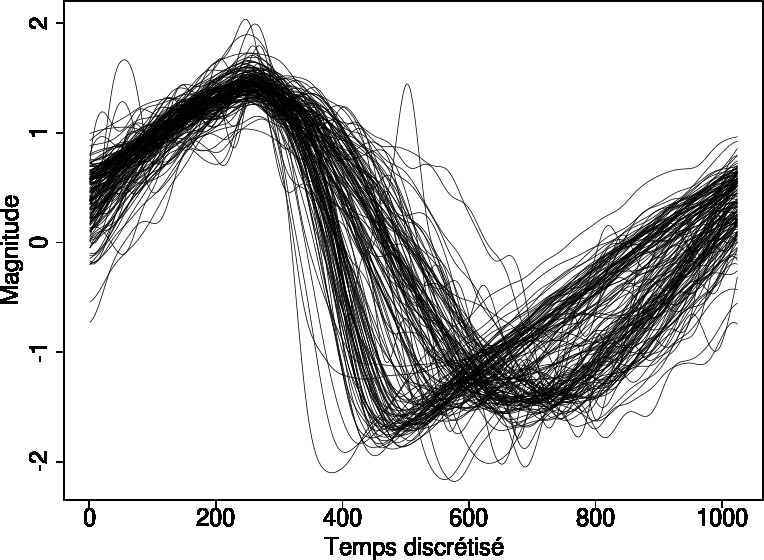
\includegraphics[width=5cm,height=3.5cm]{img/slgr1.png}
	\vspace*{-0.3cm}
	\caption{Groupe 1}
\end{minipage}
\begin{minipage}[c]{.32\linewidth}
	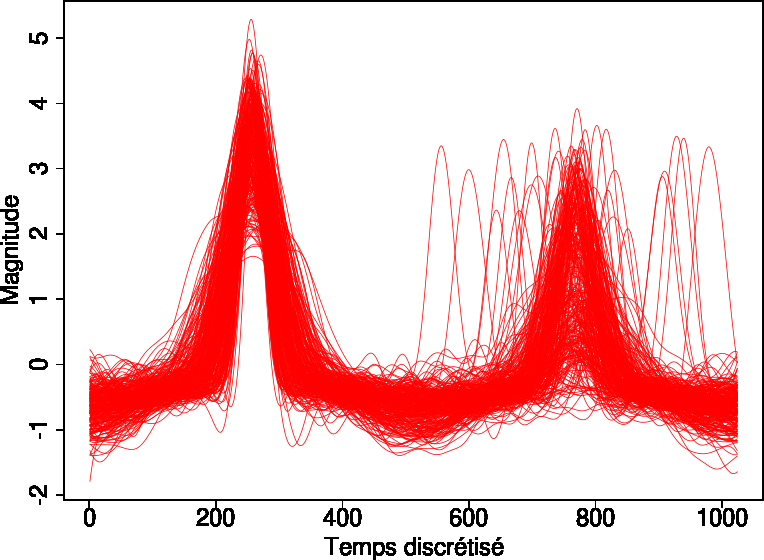
\includegraphics[width=5cm,height=3.5cm]{img/slgr2.png}
	\vspace*{-0.3cm}
	\caption{Groupe 2}
\end{minipage}
\begin{minipage}[c]{.32\linewidth}
	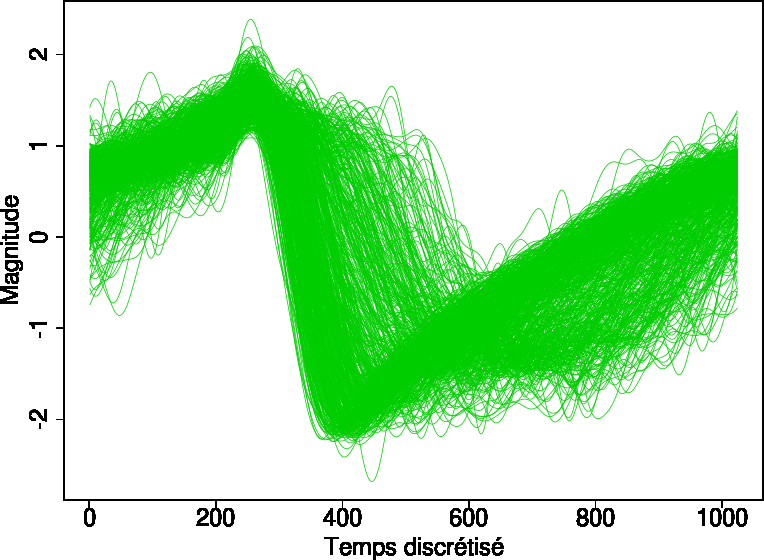
\includegraphics[width=5cm,height=3.5cm]{img/slgr3.png}
	\vspace*{-0.3cm}
	\caption{Groupe 3}
\end{minipage}
\label{figsltr3clusts}
\end{figure}

Compte-tenu du relatif faible nombre d'échantillons nous pouvons lancer le programme sur tout le jeu de données ; 
cela permet de comparer aux résultats obtenus par la version parallèle, que l'on espère presque aussi bons. 
Le tableau \ref{tabDistorSl} contient les distorsions empiriques calculées sur les ensemble d'entraînement et de test, 
ainsi que l'adéquation des deux partitions ("intra"), et leur adéquation à la partition réelle ("inter"). Cette dernière est mauvaise à cause de la remarque précitée :
les courbes des clusters 1 et 3 se ressemblent trop pour appliquer un algorithme de partitionnement de type $k$-means.\\

\begin{table}[H]
\centering
\begin{tabular}{|l|c|c|c|}
\hline
 & Distorsion & "Intra-adéquation" & "Inter-adéquation" \\
\hline
Entraînement seq. & 1.31e4 & 0.79 & 0.77\\
\hline
Entraînement // & 1.40e4 & 0.79 & 0.68\\
\hline
Test seq. & 1.09e5 & 0.78 & 0.76\\
\hline
Test // & 1.15e5 & 0.78 & 0.69\\
\hline
\end{tabular}
\caption{Distorsions et indices d'adéquation des partitions}
\label{tabDistorSl}
\end{table}

%~ 1) Starlight curves : utiliser 1000 (resp. 3000) courbes pour le clustering, puis ~9000 (resp. ~7000) pour classif.
%~ Comparer les médoïdes (renuméroter en sortie du code), et afficher les perfs : taux de classif correcte.

\subsection{Consommations électriques irlandaises}

Ce jeu de données consiste en 4621 séries temporelles représentant l'évolution de la consommation életrique d'autant de foyers irlandais. 
Celles-ci sont similaires aux courbes EDF sur lesquelles vise à être appliquée notre méthode. 
Nous avons choisi d'appliquer l'algorithme avec 3 et 5 classes. Compte-tenu du grand nombre de points de discrétisation (25k) 
et de la haute variabilité des données, celles-ci sont difficiles à représenter. Ainsi nous n'indiquons que les résultats numériques ; 
ils sont visibles dans le tableau \ref{tabDistorIr}, et sont cette fois plutôt bons.\\

\begin{table}[H]
\centering
\begin{tabular}{|l|c|c|}
\hline
 & Distorsion & "Intra-adéquation" seq. VS //\\
\hline
3 clusters seq. & 1.90e7 & 0.90\\
\hline
3 clusters // & 2.15e7 & 0.90\\
\hline
5 clusters seq. & 1.61e7 & 0.89\\
\hline
5 clusters // & 1.84e7 & 0.89\\
\hline
\end{tabular}
\caption{Distorsions et indices d'adéquation des partitions}
\label{tabDistorIr}
\end{table}
%pour un nombre de clusters égal à 3, 7 et 15.

\section{Conclusion}

Nous avons cherché à identifier des groupes de consommateurs à partir de données fonctionnelles 
pour bénéficier de l'information supplémentaire fournie par la forme des courbes, qui serait perdue 
si on les considérait comme de simples vecteurs. Cette forme est capturée $-$ entre autres caractéristiques $-$ 
par les coefficients d'ondelettes, regroupés par niveaux d'énergie. Les dissimilarités sont calculées ensuite 
via une distance $L^p$. Alternativement (ou complémentairement), il serait intéressant d'utiliser une mesure de dissimilarité 
plus directement basée sur la forme des courbes, comme le font Heckman et Zamar~(2000).\\

Ensuite, la procédure de clustering mise en place est prévue pour passer à l'échelle pour plusieurs millions de courbes. 
En effet, elle a été conçue initialement pour être appliquée aux séries temporelles des clients EDF (plusieurs dizaines de millions). 
Elle consiste à appliquer l'algorithme des $k$-médoïdes sur des groupes de courbes, puis des groupes de médoïdes 
jusqu'à obtenir un seul ensemble traité sur un processseur.
Les résultats obtenus sur les deux jeux de données présentés sont assez encourageants, et permettent d'envisager une utilisation à plus grande échelle.

%~ \section{Exemple de r\'ef\'erences bibliographiques}
%~ La n\'ecessit\'e de produire des r\'esum\'es clairs et bien
%~ r\'ef\'erenc\'es a \'et\'e d\'emontr\'ee par Achin et Quidont~(2000).
%~ Le r\'ecent article de Noteur~(2003) met en \'evidence \dots

%Quelques rappels :
%%
%\begin{center}
%%
%\begin{tabular}{lr} \hline
%%
%Accent aigu :              &  \'e; \\
%Accent grave :             &  \`a;\\
%Accent circonflexe :       &  \^o mais \^{\i};\\
%Tr\'emas :                 &  \"o mais \"{\i};\\
%C\'edille :                &  \c{c}. \\ \hline
%\end{tabular}
%%
%\end{center}

%--------------------------------------------------------------------------

\section*{Bibliographie}

\noindent [1] A. Antoniadis, X. Brossat, J. Cugliari et J.-M. Poggi (2013), Clustering Functional Data Using Wavelets, {\it International Journal of Wavelets, Multiresolution and Information Processing}, 11(1), 35--64.\\%, \texttt{doi:10.1142/S0219691313500033}
\noindent [2] R. Bekkerman, M. Bilenko et J. Langford - éditeurs (2011), Scaling up Machine Learning: Parallel and Distributed Approaches, {\it Cambridge University Press}.\\
\noindent [3] P. Berkhin (2006), A Survey of Clustering Data Mining Techniques, {\it Grouping Multidimensional Data, éditeurs : J. Kogan, C. Nicholas, M. Teboulle}.\\
\noindent [4] F. Chang, J. Dean, S. Ghemawat, W.C. Hsieh, D.A. Wallach, M. Burrows, T. Chandra, A. Fikes, et R.E. Gruber (2006), Bigtable: A Distributed Storage System for Structured Data, {\it Seventh Symposium on Operating System Design and Implementation}.\\
\noindent [5] S.-C. Chu, J.F. Roddick et J.S. Pan (2002), An Efficient K-Medoids-Based Algorithm Using Previous Medoid Index, Triangular Inequality Elimination Criteria, and Partial Distance Search, {\it Lecture Notes in Computer Science}, 2454, 63--72.\\
\noindent [6] J. Dean et S. Ghemawat (2004), MapReduce: Simplified Data Processing on Large Clusters, {\it Sixth Symposium on Operating System Design and Implementation}.\\
\noindent [7] G. De Francisci Morales et A. Bifet (2013), Introducing SAMOA, an open source platform for mining big data streams, {\it http://yahooeng.tumblr.com/post/65453012905/introducing-samoa-an-open-source-platform-for-mining}.
\noindent [8] N.E. Heckman et R.H. Zamar (2000), Comparing the shapes of regression functions. {\it Biometrika}, 87(1), 135--144.\\
\noindent [9] U. Kang, C.E. Tsourakakis et C. Faloutsos (2009), PEGASUS: A Peta-Scale Graph Mining System - Implementation and Observations, {\it IEEE International Conference on Data Mining}.\\
\noindent [10] L. Kaufman et P.J. Rousseeuw (1987), Clustering by means of Medoids, {\it Statistical Data Analysis Based on the L\_1-Norm and Related Methods, éditeur : Y. Dodge}.\\
\noindent [11] E. Keogh, Q. Zhu, B. Hu, Y. Hao, X. Xi, L. Wei et C.A. Ratanamahatana (2011), The UCR Time Series Classification/Clustering, {\it http://www.cs.ucr.edu/\~{}eamonn/time\_series\_data/}.\\
\noindent [12] R.C. Tryon (1939), Cluster analysis. {\it New York: McGraw Hill}.\\
%\noindent [7] C.C. Aggarwal - éditeur (2006) Data Streams: Models and Algorithms, \{it Advances in Database Systems}.
%[Pegasus: Mining billion-scale graphs in the cloud ? mars 2012, mais 4 pages...]
%Data Warehousing and Knowledge Discovery. 
%TODO : find paper :
%http://melmeric.files.wordpress.com/2013/04/samoa-a-platform-for-mining-big-data-streams.pdf
%http://yahooeng.tumblr.com/post/65453012905/introducing-samoa-an-open-source-platform-for-mining

%\noindent [2] Auteurs (ann\'ee), Titre, revue, localisation.
%~ \noindent [3] Achin, M. et Quidont, C. (2000), {\it Th\'eorie des
%~ Catalogues}, Editions du Soleil, Montpellier.

\end{document}

%~ Possible références :
%~ 
%~ == general
%~ 
%~ The Elements of Statistical Learning, Trevor Hastie, Robert Tibshirani, Jerome H. Friedman
%~ (14.3.10 vers page 515)
%~ 
%~ Titre	Clustering by Means of Medoids
%~ Volume 3 ;Volume 87 de Reports of the Faculty of Mathematics and Informatics. Delft University of Technology
%~ Numéro 87,Partie 3 de Reports of the Faculty of Mathematics and Informatics
%~ Auteurs	Leonard Kaufman, Peter Rousseeuw
%~ Éditeur	Fac., Univ., 1987
%~ Longueur	14 pages
%~ 
%~ Finding Groups in Data: An Introduction to Cluster Analysis (Wiley Series in Probability and Statistics) [Paperback]
%~ Leonard Kaufman (Author), Peter J. Rousseeuw (Author)
%~ 
%~ == extensions, generalisations, autres algos...
%~ 
%~ K-AP: Generating Specified K Clusters by Efficient Affinity Propagation
%~ Xiangliang Zhang, Wei Wang, Kjetil Nørvag, and Michele Sebag
%~ http://www.idi.ntnu.no/~noervaag/papers/ICDM2010.pdf
%~ 
%~ A Coherent and Heterogeneous Approach to Clustering
%~ Arian Maleki, Nima Asgharbeigi
%~ http://www.ece.rice.edu/~mam15/geo_kmedoid_AIPR08.pdf
%~ 
%~ An Efficient K-Medoids-Based Algorithm Using Previous Medoid Index, Triangular Inequality Elimination Criteria, and Partial Distance Search
%~ Shu-Chuan Chu,
%~ John F. Roddick,
%~ J. S. Pan 
%~ Data Warehousing and Knowledge Discovery
%~ Lecture Notes in Computer Science Volume 2454, 2002, pp 63-72 
%~ 
%~ http://citeseerx.ist.psu.edu/viewdoc/download?doi=10.1.1.89.3069&rep=rep1&type=pdf
%~ An efficient approach to scale up k-medoid based algorithms in large databases
%~ Maria Camila N. Barioni, Humberto L. Razente, Agma J. M. Traina, Caetano Traina Jr. ∗
%~ XXI Simpósio Brasileiro de Banco de Dados
%~ 
%~ Computational Science and Its Applications – ICCSA 2005
%~ Lecture Notes in Computer Science Volume 3482, 2005, pp 181-189
%~ A New and Efficient K-Medoid Algorithm for Spatial Clustering
    %~ Qiaoping Zhang,
    %~ Isabelle Couloigner 
%~ 
%~ == parallel
%~ 
%~ Scaling Up Machine Learning: Parallel and Distributed Approaches
%~ Ron Bekkerman, Mikhail Bilenko, John Langford
%~ 
%~ http://www.cs.umn.edu/tech_reports_upload/tr2001/01-001.pdf
%~ http://www.cs.umn.edu/research/technical_reports/view/01-001
%~ http://www.cs.cmu.edu/~lingwang/lectures/paralleldatamining2013.pdf
%~ ...
%~ 
%~ == k-medoids parallel
%~ 
%~ Parallelising the k-Medoids Clustering Problem Using Space-Partitioning
%~ Alejandro Arbelaez, Luis Quesada
%~ http://www.aaai.org/ocs/index.php/SOCS/SOCS13/paper/viewFile/7225/6231
%~ 
%~ K-Medoids: CUDA Implementation
%~ Douglas Roberts
%~ 
%~ Parallelization of K-medoid clustering algorithm 
%~ Aljoby, W. ; Queen Arwa Univ., Yemen ; Alenezi, K.
 %~ Published in:
%~ Information and Communication Technology for the Muslim World (ICT4M), 2013 5th International Conference on
%~ Date of Conference: 26-27 March 2013
%~ Page(s):
    %~ 1 - 4 
%~ Print ISBN:
    %~ 978-1-4799-0134-0 
%~ INSPEC Accession Number:
    %~ 13518450 
%~ 
%~ R package sprint
%~ http://www.ed.ac.uk/schools-departments/pathway-medicine/our-research/ghazal-group/pathway-informatics/sprint/download
%~ http://www.biomedcentral.com/1471-2105/9/558
%~ Software
%~ SPRINT: A new parallel framework for R
%~ Jon Hill1*, Matthew Hambley1, Thorsten Forster2, Muriel Mewissen2, Terence M Sloan1, Florian Scharinger1, Arthur Trew1 and Peter Ghazal2
%~ http://www.biomedcentral.com/content/pdf/1471-2105-9-558.pdf
%~ 
%~ ???
%~ 
%~ BIRCH: an efficient data clustering method for very large databases
%~ Authors: 	Tian Zhang 	Computer Sciences Dept., Univ. of Wisconsin-Madison
	%~ Raghu Ramakrishnan 	Computer Sciences Dept., Univ. of Wisconsin-Madison
	%~ Miron Livny 	Computer Sciences Dept., Univ. of Wisconsin-Madison
%~ Published in:
%~ SIGMOD '96 Proceedings of the 1996 ACM SIGMOD international conference on Management of data
%~ Pages 103-114
%~ ACM New York, NY, USA ©1996
%~ ISBN:0-89791-794-4 doi>10.1145/233269.233324
%~ 
%~ find geometric median (not medoid)
%~ http://users.jyu.fi/~samiayr/pdf/ayramo_eurogen05.pdf
%~ 
%~ ...
%~ http://citeseerx.ist.psu.edu/viewdoc/download?doi=10.1.1.110.9449&rep=rep1&type=pdf
%~ 
%~ http://biostats.bepress.com/cgi/viewcontent.cgi?article=1003&context=ucbbiostat
%~ a new PAM algo...
%~ 
%~ k-medoids initialization :
%~ http://seer.lcc.ufmg.br/index.php/jidm/article/viewFile/99/82
